\subsection{MassSpecGym - Spectrum Simulation}
{{\footnotesize
\noindent MassSpecGym curates the largest public MS/MS dataset with three standardized tasks-de novo structure 
generation, molecule retrieval, and spectrum simulation-using challenging generalization splits to 
propel ML-driven molecule discovery.


\begin{description}[labelwidth=4cm, labelsep=1em, leftmargin=4cm, itemsep=0.1em, parsep=0em]
  \item[date:] 2024-12-13
  \item[version:] v1.0
  \item[last\_updated:] 2024-12
  \item[expired:] unknown
  \item[valid:] yes
  \item[valid\_date:] 2024-12-13
  \item[url:] \href{https://neurips.cc/virtual/2024/poster/97823}{https://neurips.cc/virtual/2024/poster/97823}
  \item[doi:] unknown
  \item[domain:]
    - Chemistry
  \item[focus:] Benchmark suite for discovery and identification of molecules via MS/MS
  \item[keywords:]
    - mass spectrometry
    - molecular structure
    - de novo generation
    - retrieval
    - dataset
  \item[licensing:] unknown
  \item[task\_types:]
    - De novo generation
    - Retrieval
    - Simulation
  \item[ai\_capability\_measured:]
    - Molecular identification and generation from spectral data
  \item[metrics:]
    - Structure accuracy
    - Retrieval precision
    - Simulation MSE
  \item[models:]
    - Graph-based generative models
    - Retrieval baselines
  \item[ml\_motif:]
    - Regression
  \item[type:] Dataset, Benchmark
  \item[ml\_task:]
    - Generation, retrieval, simulation
  \item[solutions:] 0
  \item[notes:] Dataset\textasciitilde{}>1M spectra; open-source GitHub repo; widely cited as a go-to benchmark for MS/MS tasks.

  \item[contact.name:] Roman Bushuiev
  \item[contact.email:] unknown
  \item[results.links.name:] ChatGPT LLM
  \item[fair.reproducible:] Yes
  \item[fair.benchmark\_ready:] Yes
  \item[id:] massspecgym\_-\_spectrum\_simulation
  \item[Citations:] \cite{neurips2024_c6c31413}
\end{description}

{\bf Ratings:} ~ \\

\begin{tabular}{p{0.15\textwidth} p{0.07\textwidth} p{0.7\textwidth}}
\hline
Rating & Value & Reason \\
\hline
dataset & 5 & Largest public MS/MS dataset with extensive annotations; minor point deducted for
lack of explicit train/validation/test splits.
 \\
documentation & 1 & Paper and poster describe benchmark goals and design, but documentation and user
guides are minimal and repo status uncertain.
 \\
metrics & 5 & Well-defined metrics such as structure accuracy, retrieval precision, and simulation MSE
used consistently.
 \\
reference\_solution & 3.5 & CNN-based baselines are referenced, but pretrained weights and comprehensive training
pipelines are not fully documented.
 \\
software & 3 & Open-source GitHub repository available; baseline models and training code partially
provided but overall framework maturity is moderate.
 \\
specification & 5 & Clearly defined tasks including molecule generation, retrieval, and spectrum simulation,
scoped for MS/MS molecular identification.
 \\
\hline
\end{tabular}

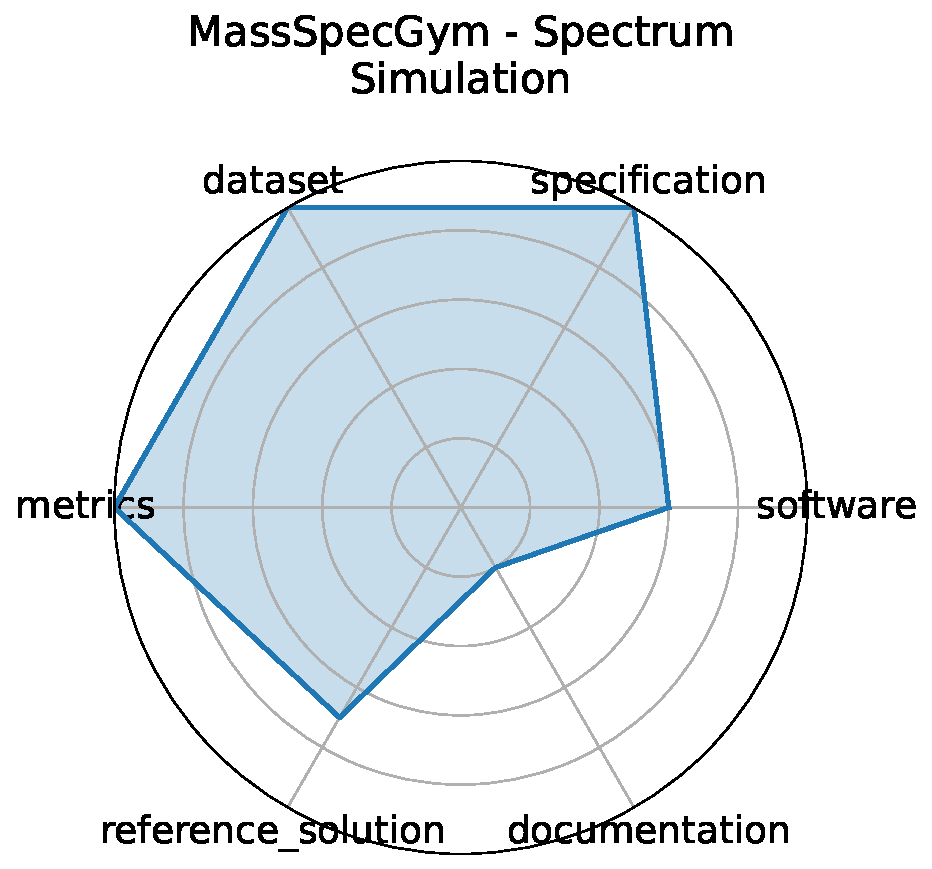
\includegraphics[width=0.2\textwidth]{massspecgym_-_spectrum_simulation_radar.pdf}
}}
\clearpage